Современная задача оптимизации с учетом
случайности в данных обучения записывается как \cite{nesterov2015universal}:
\begin{equation}
    f(x) = \mathrm{E} f(x,\xi) \rightarrow \min_x,
\end{equation}
где пара $(x,\xi)$ является результатом наблюдения.
В секции будут разобраны только методы порядка.

\text{Определение} Фукнция $f$ называется $L$-липшицевой для метрики $\rho$, 
если $\forall x,y \rightarrow \rho(f(x),f(y)) \le L \cdot \rho(x,y)$.
Для оптимизации в качестве метрики как правило выбирают $\rho(x,y) =\|x-y \|^2$:   
\begin{equation}
    |f(x) - f(y)| \le L \cdot |x-y|^2
\end{equation}

\textit{Определение} $\mu$ -гладкой называется f(X) функция,для которой выполнено \begin{equation}
   \forall x_1,x_2 \in S \rightarrow f(\lambda x_1 + (1-\lambda)x_2) \le \lambda f(x_1) + (1-\lambda) f(x_2) - \frac{\mu}{2} \lambda (1-\lambda) \| x_1 - x_2 \|^2,
\end{equation}
где $S$ - выпуклое множество и $\mu > 0$. 

\begin{figure}[h]
    \centering
    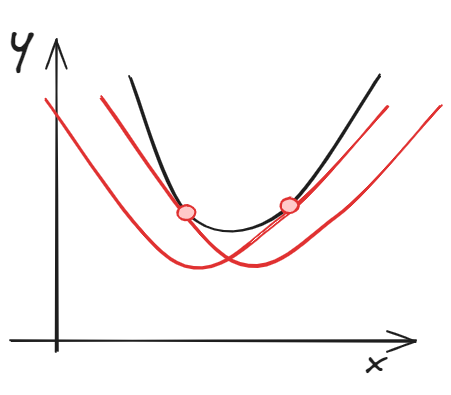
\includegraphics[width=0.5\textwidth]{assets/math/optimization/strong_convex.excalidraw.png}
    \caption{Сильная выпуклость позволяет выполнить квадратичную оценку снизу}
    \label{strong_convex}
\end{figure}

Для выпуклых функций справедливо неравенство Йенсена
\begin{equation}
    f \left( \sum_{i=1}^k \alpha_i x_i \right) = \sum_{i=1}^k \alpha_i f(x_i),
\end{equation}
причем равенство выполняется только при $x_1 = \dots =x_k$.

Практически важным для выпуклой функции является результат для ее матождидания:
\begin{equation}
    f(\mathbb{E} X) \le \mathbb{E} f(X)
\end{equation}

Кубическая регуляризация \cite{}

\textit{Определение} \textbf{Усредненным по подвыборке} мощностью $B$ стохастическим градиентом называется 
$\nabla^B f(x,\xi) = \sum_{j=i}^B \nabla f(x,\xi_i)$.

